\documentclass[12pt, a4paper, simple]{eskdtext}

\usepackage{_STYLES/title_variables}
\usepackage{_STYLES/eskd_variables}
\usepackage{_STYLES/listings}
\usepackage{_STYLES/tableOfContent}
\usepackage{_STYLES/pictures}
\usepackage{_STYLES/tables}
\usepackage{_STYLES/url}
\usepackage{pgfplots}
\pgfplotsset{compat=newest}

% Графа 1 (наименование изделия/документа)
\ESKDcolumnI{\ESKDfontIII\titlePageTopic\\Пояснительная записка}

% Графа 2 (обозначение документа)
% AA.BBB.CCCCCC-DD EE FF
\ESKDsignature{КР.ПО4.\titlePageStudentCreditCard-0\titlePageNumberWork~81~00}
% AA - тип работы
% BBB - группа
% СССССС - номер зачётки
% DD - номер работы
% EE - тип документа
% FF - версия документа

\begin{document}
    % Титульная страница
    \begin{ESKDtitlePage}
        \begin{center}
    МИНИСТЕРСТВО ОБРАЗОВАНИЯ РЕСПУБЛИКИ БЕЛАРУСЬ
    
    \hspace{0pt}

    УЧРЕЖДЕНИЕ ОБРАЗОВАНИЯ

    <<БРЕСТСКИЙ ГОСУДАРСТВЕННЫЙ ТЕХНИЧЕСКИЙ УНИВЕРСИТЕТ>>

    \hspace{0pt}

    КАФЕДРА \titlePageKafedra
\end{center}

\vfill

\begin{center}
    \titlePageTopic

    \hspace{0pt}

    ПОЯСНИТЕЛЬНАЯ ЗАПИСКА К КУРСОВОЙ РАБОТЕ

    ПО ДИСЦИПЛИНЕ <<\titlePageDistiplina>>
\end{center}

\vfill

\begin{center}
    % AA.BBB.CCCCCC-DD EE FF
    КР.ПО4.\titlePageStudentCreditCard-0\titlePageNumberWork~81~00
    % AA - тип работы
    % BBB - группа
    % СССССС - номер зачётки
    % DD - номер работы
    % EE - тип документа
    % FF - версия документа

    \hspace{0pt}

    Листов \pageref{LastPage}
\end{center}

\vfill

\begin{flushright}
    \begin{minipage}[t]{.49\textwidth}
        \begin{minipage}[t]{.75\textwidth}
            \begin{flushright}
                Руководитель

                Выполнил

                Консультант

                по ЕСПД
            \end{flushright}
        \end{minipage}
    \end{minipage}
    \begin{minipage}[t]{.49\textwidth}
        \begin{flushright}
            \begin{minipage}[t]{.75\textwidth}
                \titlePageLeaderName~\titlePageLeaderSurname

                \titlePageAuthorName~\titlePageAuthorSurname

                \hspace{0pt}

                \titlePageConsultantName~\titlePageConsultantSurname

            \end{minipage}
        \end{flushright}
        
    \end{minipage}
\end{flushright}

\vfill

\begin{center}
    \ESKDtheYear
\end{center}
    \end{ESKDtitlePage}

    % ТЗ
    \ESKDthisStyle{empty}
    Здесь лист с ТЗ.
    \newpage
    \ESKDthisStyle{formII}

    % Содержание
    \tableofcontents
    \paragraph{Приложение А. Текст программы}
    \paragraph{Приложение Б. Схема алгоритма}
    \newpage

    \section*{ВВЕДЕНИЕ} % Секция без номера
\addcontentsline{toc}{section}{ВВЕДЕНИЕ} % Добавить в содержание
 \newpage
    \section{Постановка задачи}

Требуется

\begin{enumerate}
    \item[1)] выполнить создание и обучение моделей нейронных сетей на базе вышеуказанного фреймворка, задача: распознование рупописных символов на основе БД MNIST;
    \item[2)] исследовать производительность, точность обучения и распознавания рукописных цифр на базе полученных модулей;
    \item[3)] задачи 1 и 2 выполнить для различных конфигураций нейронных сетей;
    \item[4)] выполнить сравнительный анализ полученных моделей.
\end{enumerate} \newpage
    \section{Анализ и описание используемого фреймворка}

\subsection{TensorFlow}

\subsubsection{История}
TensorFlow - открытая программная библиотека для машинного обучения,
разработанная компанией Google для решения задач построения и тренировки нейронной сети
с целью автоматического нахождения и классификации образов,
достигая качества человеческого восприятия.
Применяется как для исследований,
так и для разработки собственных продуктов Google.
Основной API для работы с библиотекой реализован для Python,
также существуют реализации для R, C Sharp, C++, Haskell, Java, Go и Swift.

Является продолжением закрытого проекта DistBelief.
Изначально TensorFlow была разработана командой Google Brain для внутреннего использования в Google,
в 2015 году система была переведена в свободный доступ с открытой лицензией Apache 2.0. 

\subsubsection{Лицензия}
TensorFlow доступна по лицензии Apache License 2.0.
Это дает нам возможность редактировать сам фреймворк.
В ходе курсового проекта нам не понадобится редактировать фреймворк.

\subsubsection{Операционная система}
TensorFlow доступен на разных операционных системах:
Windows, Android, iOS, Linux, MaсOS.
В ходе курсового проекта была выбрана операционная система Linux Debian 10 Xfce.

\subsubsection{Язык}
Чтобы писать на TensorFlow мы можем использовать выскоуровневые языки
такие как C++, Python, JavaScript.
В ходе курсового проекта был выбран язык Python.

\subsubsection{Версия}
Последняя версия TensorFlow имеет версию 2.5.0.

Узнать версию можем через \verb|tensorflow.__version__|.

\begin{lstlisting}[language=Python,]
    import tensorflow
    print(f'TensorFlow verion : {tensorflow.__version__}')
\end{lstlisting}

С версии 2.0 TensofFlow использует GPU.
То есть на Windows, Linux требуется ещё устанавливать CUDA for CPU TensorFlow.
TensorFlow можно запустить в двух режимах:
1) c поддержкой графического процессора,
2) без поддержки графического процессора.

Для такого, чтобы включить поддержку графического процессора,
то в Python используем библиотеку os.

\begin{lstlisting}[language=Python,]
    import os
    os.environ['TF_CPP_MIN_LOG_LEVEL'] = '2'
\end{lstlisting}

\subsection{Keras}

\subsubsection{История}
Keras - открытая нейросетевая библиотека,
написанная на языке Python.
Она представляет собой надстройку над фреймворками
Deeplearning4j, TensorFlow и Theano.
Нацелена на оперативную работу с сетями глубинного обучения,
при этом спроектирована так,
чтобы быть компактной,
модульной и расширяемой.
Она была создана как часть исследовательских усилий проекта ONEIROS
(англ. Open-ended Neuro-Electronic Intelligent Robot Operating System),
а ее основным автором и поддерживающим является Франсуа Шолле
(фр. François Chollet), инженер Google.

TensorFlow является фреймворком низкоуровневым.
Один разработчик Google написал свою надстройку Keras.
В итоге Google внедрила keras в сам tensorflow.
В ходе курсового проекта для удобства моделирования будет использоваться надстройка Keras.

\subsubsection{Лицензия}
Keras доступен по лицензии MIT. То есть мы имеем полное право её модифицировать. Но в ходе курсового проекта нам этого делать не прийдется.

\subsubsection{Операционная система}
Keras является мультиплатфоренный.
Так как мы используем Linux,
то библиотека для курсового проекта нам подходит.

\subsubsection{Язык}
Keras остается нашей библиотекой для фреймворка TensorFlow.
В ходе курсового проекта выбран высоко уровневый язык Python.
То есть Keras также будем использовать в Python.

\subsubsection{Версия}
Так как Keras мы используем как библиотеку включенную поумолчанию в TensorFlow,
то версия Keras совпадает с версией TensorFlow.

Узнать версию можем через \verb|tensorflow.keras.__verison__|.

\begin{lstlisting}[language=Python,]
    from tensorflow import keras
    print(f'Keras verion : {tensorflow.keras.__version__}')
\end{lstlisting} \newpage
    \section{Моделирование нейронных сетей и алгоритмов обучения}
 \newpage
    \section{Разработка и описание программных модулей}



\subsection{Jupyter Notebook}

При написании кода приходится при каждом запуске скрипта Python,
снова начитатся обучать нейронная сеть.
Чтобы такого небыло можно поблочно выполнять, перевыполнять Python код в Jupyter Notebook.
Скриншот Jupyter Notebook на
рисунке~\textbf{\ref{fig:4_JupyterNotebook} (стр. \pageref{fig:4_JupyterNotebook})}.

\begin{figure}[!htbp]
    \centering
    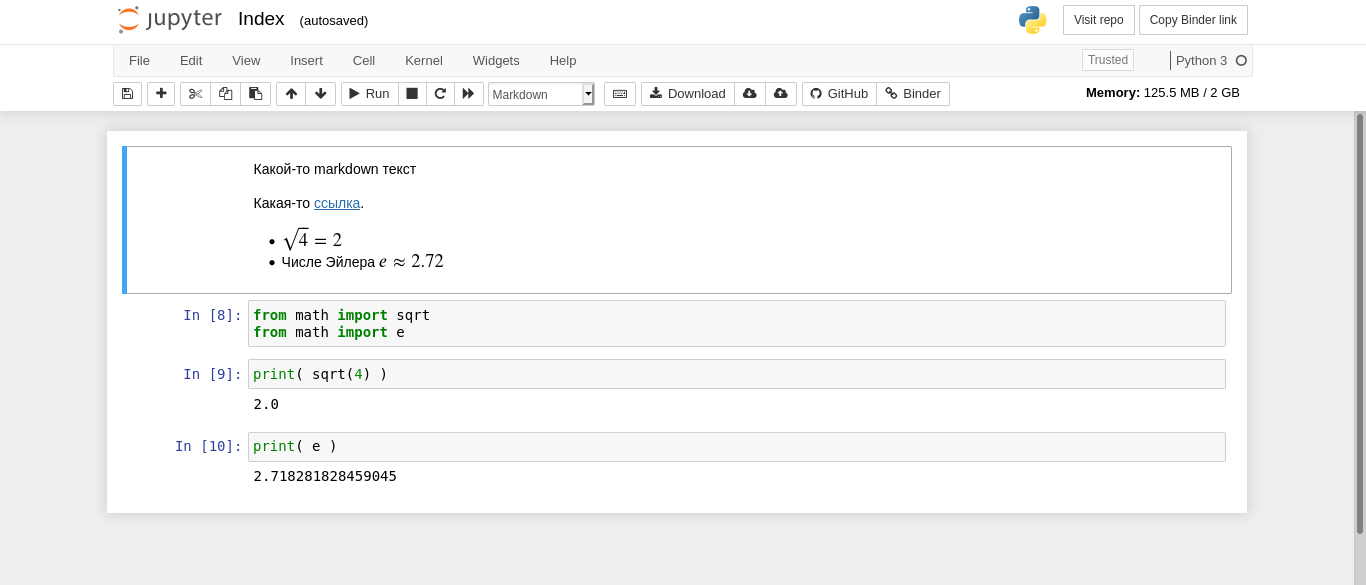
\includegraphics[width=16cm]
    {_INCLUDES/main/4/JupyterNotebook.png}
    \caption{Jupyter Notebook}
    \label{fig:4_JupyterNotebook}
\end{figure}



\subsection{Google Colaboratory}

Jupyter Notebook - это удобно, но пользуя веб версией мы не получаем все библиотеки Python.
В итоге приходится скачивать Jupyter Notebook на компьютер и ручками скачивать библиотеки,
такие как numpy и tensorflow. Также для обучения нейронной сети на tensorflow нужен графический процессор. Эти две проблемы решает Google Colaboratory, который содержит различные библиотеки Python и дает доступ к другой машине, которая будет обучать нейронную сеть даже с телефона.
Скриншот Google Colaboratory на
рисунке~\textbf{\ref{fig:4_GoogleColaboratory} (стр. \pageref{fig:4_GoogleColaboratory})}.

\begin{figure}[!htbp]
    \centering
    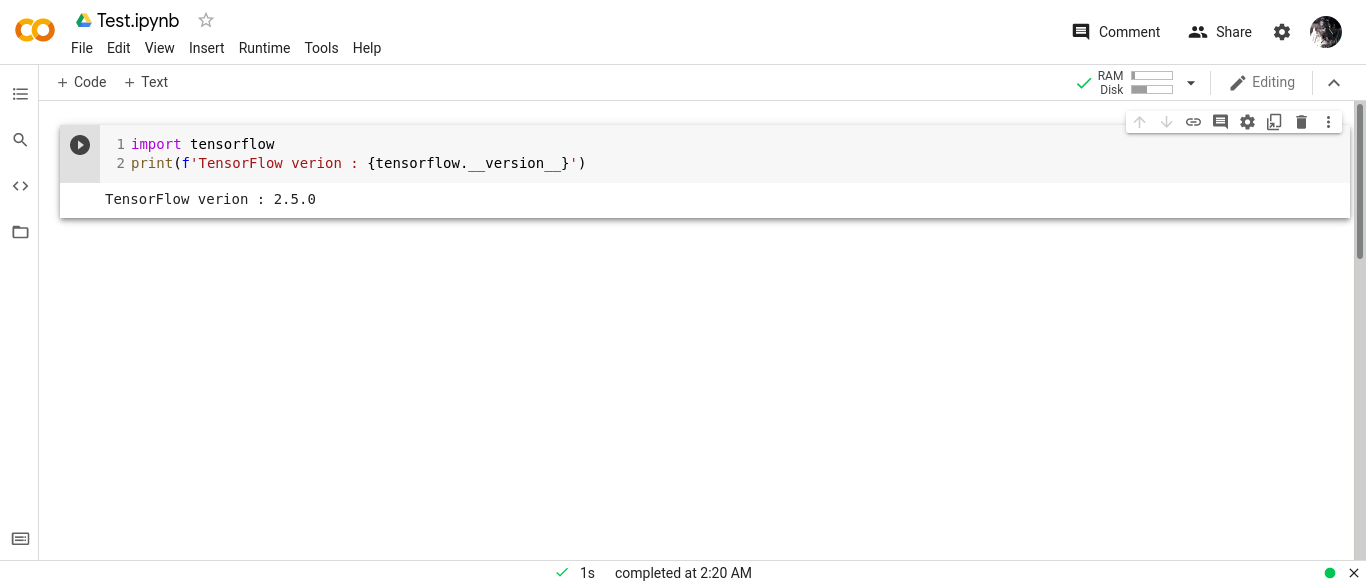
\includegraphics[width=16cm]
    {_INCLUDES/main/4/GoogleColaboratory.png}
    \caption{Google Colaboratory}
    \label{fig:4_GoogleColaboratory}
\end{figure}



\subsection{Google Colaboratory секции}



\subsubsection{Секция библиотек}

В секции библиотек подключаем следующие библиотеки:

\begin{enumerate}
    \item numpy - для создания массивов
    \item matplotlib.pyplot - для рисования графиков и картинок
    \item tensorflow - фреймворк
\end{enumerate}

\begin{lstlisting}[language=Python,]
    import numpy as np
    import matplotlib.pyplot as plt
    import tensorflow
\end{lstlisting}



\subsubsection{Секция загрузки БД mnist}

\subparagraph{Функция tensorflow.keras.datasets.mnist.load\_data()} \hspace{0pt}

\underline{Входные параметры}: нет.

\underline{Назначение}: загружает в кортедж кортеджей картинки и результат картинок для обучающей и тестовой выборки.

\underline{Возвращаемые данные}: кортедж кортеджей.

\begin{lstlisting}[language=Python,]
    (x_train, y_train), (x_test, y_test) = tensorflow.keras.datasets.mnist.load_data()
\end{lstlisting}

Где <<\verb|x_train|>> - изображения цифр обучающей выборки.

Где <<\verb|у_train|>> - вектор соответсвующих значений цифр,
если на i-отом изображении нарисовано 5, то \verb|y_train[i] = 5|.

Где <<\verb|x_test|>> - изображения цифр тестовой выборки.

Где <<\verb|у_test|>> - вектор соответствующих значений цифр для тестовой выборки,
если на i-отом изображении нарисовано 5, то \verb|y_test[i] = 5|.



\subsubsection{Секция нормирования входных параметров}

В базе данных MNIST изображения рукописных цифр черно-белые. Преобразовав изображения в массив мы имеем градацию цветов в диапазоне от единицы до 255. Максимальное число 255. Если мы разделим каждый пиксель на 255, то получим массив из значение не от 1 до 255, а со значениями от нуля до единицы, которые можем подавать на входные нейроны.

\begin{lstlisting}[language=Python,]
    # стандартизация входных данных
    x_train = x_train / 255
    x_test = x_test / 255
\end{lstlisting}



\newpage



\subsubsection{Секция классификации выходного слоя}

\subparagraph{Функция tensorflow.keras.datasets.mnist.load\_data()} \hspace{0pt}

\underline{Входные параметры}:

\begin{enumerate}
    \item y - массив чисел
    \item num\_classes - количество классов
\end{enumerate}

\underline{Назначение}: создаст массив размером num\_classes, в который под цифрой запишет 1.

Например, если это число 0, то массив [1,0,0,0,0,0,0,0,0,0].

Например, если это число 1, то массив [0,1,0,0,0,0,0,0,0,0].

Например, если это число 2, то массив [0,0,1,0,0,0,0,0,0,0].

Например, если это число 3, то массив [0,0,0,1,0,0,0,0,0,0].

Например, если это число 4, то массив [0,0,0,0,1,0,0,0,0,0].

Например, если это число 5, то массив [0,0,0,0,0,1,0,0,0,0].

Например, если это число 6, то массив [0,0,0,0,0,0,1,0,0,0].

Например, если это число 7, то массив [0,0,0,0,0,0,0,1,0,0].

Например, если это число 8, то массив [0,0,0,0,0,0,0,0,1,0].

Например, если это число 9, то массив [0,0,0,0,0,0,0,0,0,1].

\underline{Возвращаемые данные}: кортедж кортеджей.

\begin{lstlisting}[language=Python,]
    y_train_cat = tensorflow.keras.utils.to_categorical(y_train, 10)
    y_test_cat = tensorflow.keras.utils.to_categorical(y_test, 10)
\end{lstlisting}



\subsubsection{Секция печати картинок обучающей выборки}

Печатаем 200 картинок обучающей выборки.

\begin{lstlisting}[language=Python,]
    # отображение первых 20*24=480 изображений из обучающей выборки
    plt.figure(figsize=(10,14)) # размер в дюймах
    for i in range(480):
        plt.subplot(20,24,i+1)  # картинки 20 по строке и 24 по столбцу
        plt.xticks([])          # не печатать оси по x
        plt.yticks([])          # не печатать оси по y
        plt.title(y_train[i])   # печатать в заголовке картинки цифру
        plt.imshow(             # печатать в рамке картинку
            x_train[i],
            cmap=plt.cm.binary
        )  
    plt.show()                  # печатаем картинку в окно
\end{lstlisting}

Результат на рисунке~\textbf{\ref{fig:4_x_train} (стр. \pageref{fig:4_x_train})}.

\begin{figure}[!htbp]
    \centering
    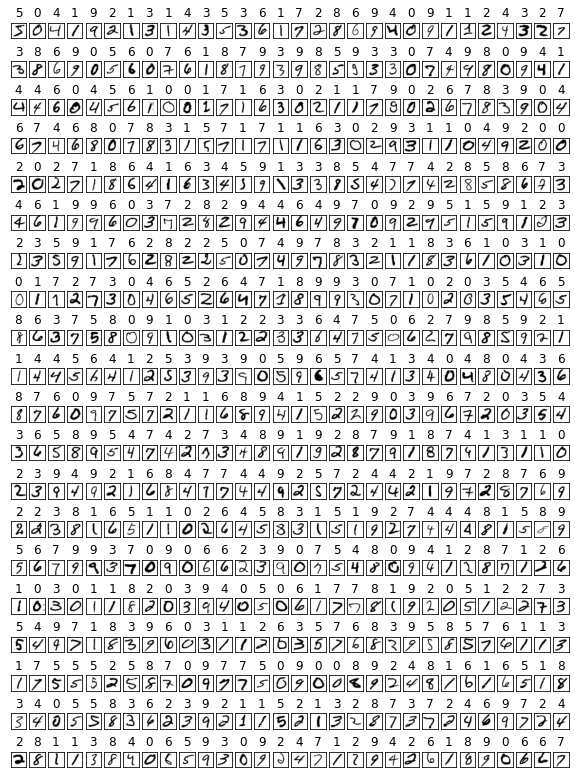
\includegraphics[width=14.6cm]
    {_INCLUDES/main/4/x_train.png}
    \caption{Выборка цифр}
    \label{fig:4_x_train}
\end{figure}



\subsubsection{Секция моделирования нейронной сети}


\subparagraph{Функция keras.Sequential} \hspace{0pt}

\underline{Входные параметры}: список слоев нейронной сети.

\underline{Назначение}: создает объект модель нейронной сети, у которой появляються методы.

\underline{Возвращаемые данные}: object - объект модели.

\subparagraph{} \hspace{0pt}

Flatten - создает слой, который будет брать значения пикселей картинки построчно.

Dense - создаёт слой, который связывает нейронны предыдущего слоя с текущим.

\begin{lstlisting}[language=Python,]
    model = tensorflow.keras.Sequential([
        tensorflow.keras.layers.Flatten(input_shape=(28, 28, 1)),
        tensorflow.keras.layers.Dense(128, activation='relu'),
        tensorflow.keras.layers.Dense(10, activation='softmax')
    ])
\end{lstlisting}

\subparagraph{Метод .summary} \hspace{0pt}

\underline{Входные параметры}: нет.

\underline{Назначение}: печатает характеристики созданной модели.

\underline{Возвращаемые данные}: None.


\begin{lstlisting}[language=Python,]
    print( model.summary() )
\end{lstlisting}



\subsubsection{Секция компиляции нейронной сети}

\subparagraph{Метод .compile} \hspace{0pt}

\underline{Входные параметры}:
\begin{enumerate}
    \item (необязательный) optimizer - тип оптимизации;
    \item (необязательный) loss - функция потерь;
    \item (необязательный) metrics - метрика.
\end{enumerate}

\underline{Назначение}: компилирует нейронную сеть.

\underline{Возвращаемые данные}: None.

\begin{lstlisting}[language=Python,]
    model.compile(
        #optimizer='adam',
        optimizer=tensorflow.keras.optimizers.Adam(0.001),
        loss='categorical_crossentropy',
        metrics=['accuracy']
    )
\end{lstlisting}



\subsubsection{Секция обучения нейронной сети}


\subparagraph{Метод .fit} \hspace{0pt}

\underline{Входные параметры}:
\begin{enumerate}
    \item x\_train - входное обучающее множество;
    \item y\_train\_cat - требуемые значения на выходе;
    \item (необязательный) batch\_size - размер batch'a (после скольки изображений будет меняться веса);
    \item (необязательный) epochs - количество эпох;
    \item (необязательный) validation\_split - разбиение обучающей выборки.
\end{enumerate}

\underline{Назначение}: выводит информацию при обучении на каждой эпохе.

\underline{Возвращаемые данные}: object.

\begin{lstlisting}[language=Python,]
    model.fit(
        x_train,
        y_train_cat,
        batch_size=32,
        epochs=5,
        validation_split=0.2
    )
\end{lstlisting}



\newpage



\subsubsection{Секция оценки качества нейронной сети на тестовой выборке}

\subparagraph{Метод .evaluate} \hspace{0pt}

\underline{Входные параметры}:
\begin{enumerate}
    \item x\_test - картинки тестовой выборки;
    \item y\_test\_cat - ожидаемый результат тестовой выборки.
\end{enumerate}

\underline{Назначение}: выводит в списке значение потерь и значение показатель обучения.

\underline{Возвращаемые данные}: list - список.

\begin{lstlisting}[language=Python,]
    model.evaluate(x_test, y_test_cat)
\end{lstlisting}

\begin{lstlisting}[name=Вывод в консоль,]
    [0.12078429013490677, 0.9781000018119812]
\end{lstlisting}



\subsubsection{Секция вывода пердсказанного числа и картинки}

\subparagraph{Функция print\_info\_about\_image\_by\_index(n)} \hspace{0pt}

\underline{Входные параметры}: n - индекс картинки.

\underline{Назначение}: выводит картинку, а в заголовке предсказанное значение.

\underline{Возвращаемые данные}: нет.

\begin{lstlisting}[language=Python,]
    def print_info_about_image_by_index(n):
        x = numpy.expand_dims( x_test[n], axis=0 )
        res = model.predict(x)
        print(f'Десять выходных значений: {res}')
        print(f'Распознанная цифра : {numpy.argmax(res)}')
        print()
        plt.imshow(x_test[n], cmap=plt.cm.binary)
        plt.show()
\end{lstlisting}

\begin{lstlisting}[language=Python,]
    # 10 раз вызвали функцию
    for i in range(0, 10):
        print_info_about_image_by_index(i)
\end{lstlisting}

Результат на
рисунке~\textbf{\ref{fig:4_img_and_result} (стр. \pageref{fig:4_img_and_result})}.

\begin{figure}[!htp]
    \centering

    \begin{minipage}[h]{0.19\linewidth}
        \centering
        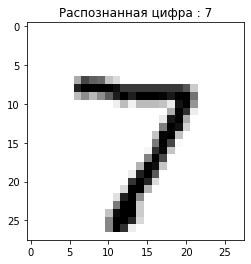
\includegraphics[width=\linewidth]
        {_INCLUDES/main/4/result1.png}
    \end{minipage}
    \hfill
    \begin{minipage}[h]{0.19\linewidth}
        \centering
        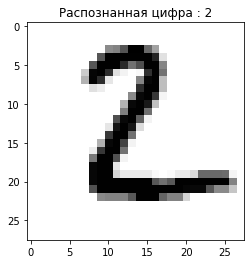
\includegraphics[width=\linewidth]
        {_INCLUDES/main/4/result2.png}
    \end{minipage}
    \hfill
    \begin{minipage}[h]{0.19\linewidth}
        \centering
        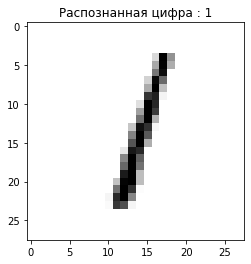
\includegraphics[width=\linewidth]
        {_INCLUDES/main/4/result3.png}
    \end{minipage}
    \hfill
    \begin{minipage}[h]{0.19\linewidth}
        \centering
        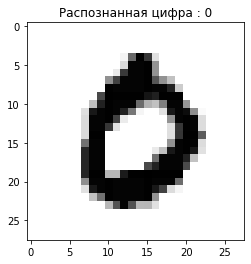
\includegraphics[width=\linewidth]
        {_INCLUDES/main/4/result4.png}
    \end{minipage}
    \hfill
    \begin{minipage}[h]{0.19\linewidth}
        \centering
        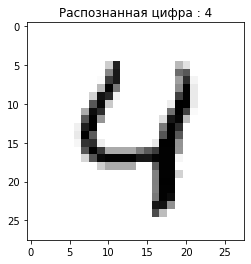
\includegraphics[width=\linewidth]
        {_INCLUDES/main/4/result5.png}
    \end{minipage}


    \begin{minipage}[h]{0.19\linewidth}
        \centering
        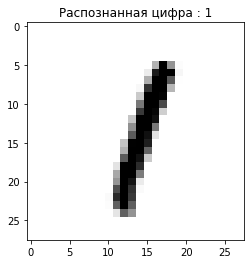
\includegraphics[width=\linewidth]
        {_INCLUDES/main/4/result6.png}
    \end{minipage}
    \hfill
    \begin{minipage}[h]{0.19\linewidth}
        \centering
        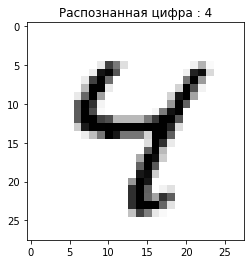
\includegraphics[width=\linewidth]
        {_INCLUDES/main/4/result7.png}
    \end{minipage}
    \hfill
    \begin{minipage}[h]{0.19\linewidth}
        \centering
        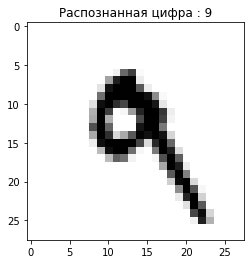
\includegraphics[width=\linewidth]
        {_INCLUDES/main/4/result8.png}
    \end{minipage}
    \hfill
    \begin{minipage}[h]{0.19\linewidth}
        \centering
        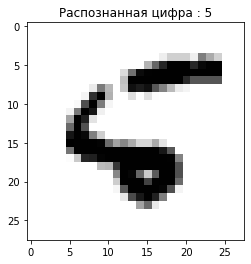
\includegraphics[width=\linewidth]
        {_INCLUDES/main/4/result9.png}
    \end{minipage}
    \hfill
    \begin{minipage}[h]{0.19\linewidth}
        \centering
        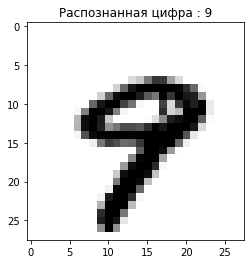
\includegraphics[width=\linewidth]
        {_INCLUDES/main/4/result10.png}
    \end{minipage}

    \caption{Картинка и результат нейронной сети}
    \label{fig:4_img_and_result}
\end{figure}



\subsubsection{Отбор неправильно распознанных изображений}

При тестировании у нас есть уже какие-то ответы нейронной сети. То что изображено на картинке мы также знаем. Если то, что изображено на картинке совпадает с результатом выданным нейронной сетью, то добавляем в массив True, иначе False. Неправльно распознанные изображения у нас с меткой False. С помощью маски мы отбираем неправильные изображения.

\begin{lstlisting}[language=Python,]
    mask = pred == y_test
    x_false = x_test[~mask]
    p_false = pred[~mask]
    print(f'Размерность x_false : {x_false.shape}')
    print(f'Размерность p_false : {p_false.shape}')
\end{lstlisting}

\begin{lstlisting}[name=Вывод в консоль,]
    Размерность x_false : (243, 28, 28)
    Размерность p_false : (243,)
\end{lstlisting}

В итоге сеть не распознала 243 изображения.



\newpage



\subsubsection{Вывод неправильных картинок}

\begin{lstlisting}[language=Python,]
    # Вывод первых 243 неверных результатов
    plt.figure(figsize=(10,10)) # размер в дюймах
    for i in range(243):
        plt.subplot(13,20,i+1)  # расположить картинки в 13x20
        plt.xticks([])          # не выводить оси по x
        plt.yticks([])          # не выводить оси по y
        plt.title(p_false[i])   # печать в заголовок картинки цифру
        plt.imshow(x_false[i], cmap=plt.cm.binary) # печатает в рамку
    plt.show()                  # напечатать картинку
\end{lstlisting}

Не правильно распознанные картинки изображены на
рисунке~\textbf{\ref{fig:4_not_right_imgs} (стр. \pageref{fig:4_not_right_imgs})}.

\begin{figure}[!htbp]
    \centering
    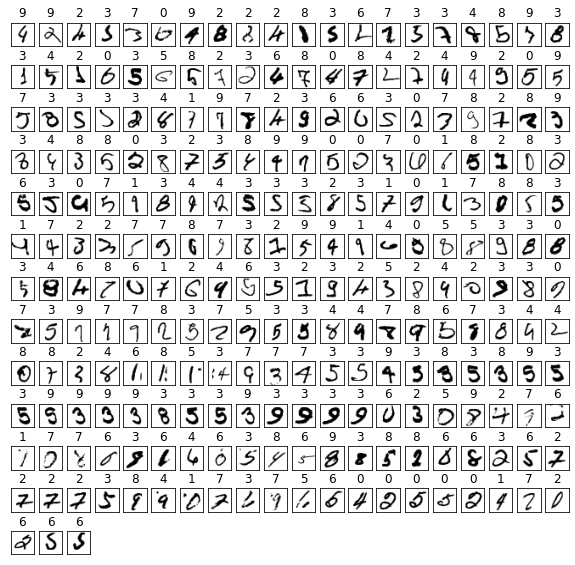
\includegraphics[width=14cm]
    {_INCLUDES/main/4/not_right_imgs.png}
    \caption{Не правльно распознанные цифры}
    \label{fig:4_not_right_imgs}
\end{figure} \newpage
    \section{Тестирование, сравнительный анализ и результаты исследования}
 \newpage
    \section{Заключение}

Нейронные сети, технологии прошлого века, меняют работу целых отраслей. Одни возмодности нейронной сети поражают, а другие заставляют задуматься в их пользу как специалистов.

В результате курсового проекта была разработана нейронная сеть,
которая распознает рукописные цифры базы данных MNIST,
написанная на tensorflow,
которая использует надстройку Keras.

Архитектура сети представлена на листинге.

\begin{lstlisting}[language=Python]
    model = tensorflow.keras.Sequential([
        tensorflow.keras.layers.Flatten(input_shape=(28, 28, 1)),
        tensorflow.keras.layers.Dense(128, activation='relu'),
        tensorflow.keras.layers.Dense(10, activation='softmax')
    ])

    model.compile(
        optimizer=tensorflow.keras.optimizers.Adam(0.001),
        loss='categorical_crossentropy',
        metrics=['accuracy']
    )
\end{lstlisting} \newpage
    \newpage

\begingroup
  \section*{СПИСОК ИСПОЛЬЗОВАННЫХ ИСТОЧНИКОВ}
  \phantomsection
  \addcontentsline{toc}{section}{СПИСОК ИСПОЛЬЗОВАННЫХ ИСТОЧНИКОВ}

  \renewcommand{\addcontentsline}[3]{}% Remove functionality of \addcontentsline
  \renewcommand{\section}[2]{}% Remove functionality of \section

  \begin{thebibliography}{}
	\bibitem{youtube_start_learn_nn}
	Как я начал изучать нейросети и python - YouTube
	[Электронный ресурс].
	Режим доступа: \url{https://www.youtube.com/watch?v=PHdw0Uk_Lc4}.

	\bibitem{youtube_keras_7}
	Keras - установка и первое знакомство | \#7 нейросети на Python - YouTube
	[Электронный ресурс].
	Режим доступа: \url{https://www.youtube.com/watch?v=BQg9OZdzLLE}.

    \bibitem{youtube_start_learn_nn}
	Keras - обучение сети распознаванию рукописных цифр | \#8 нейросети на Python - YouTube
	[Электронный ресурс].\\
	Режим доступа: \url{https://www.youtube.com/watch?v=oCXh_GFMmOE}.

	\bibitem{moreDomains}
	Как нейронная сеть распознает цифры | \#9 нейросети на Python - YouTube
	[Электронный ресурс].
	Режим доступа: \url{https://www.youtube.com/watch?v=S3cViFMiYZ4}.
  \end{thebibliography}
\endgroup

\newpage

\end{document}